% Chapter 2

\chapter{方案设计}

\section{概要}
设计要求是:用户输入一张图片后,可以得到相应的标注语句,了解图片语义;在用户输入一句话的时候,可以得到描述这一句话的图片,直观“感受”文字。

软件设计主界面使用python的tkinter包来制作。python是一个跨平台语言,用python制作方便产品在不同平台使用。界面中应当可以选择调动两个功能,分别是图片翻译为自然语言和语句翻译为图片。两个功能分别提前训练出成品模型,通过主界面按钮内嵌入的方法,调用对应模型进行计算。

\section{软件模型}
软件分为三个部分,第一部分是软件界面,需要实现简洁明了的操作功能,方便使用。

第二部分是图片标注功能。实现这一功能的模型通过image caption的模型进行训练,算法参照蒙特利尔大学Kevin Xu\upcite{xu2015show}提出的模型进行实现,并经过基于一个或多个数据集进行多个epoch的训练,比较选出表现较好的模型,嵌入到应用中使用。

第三部分是文本生成图片功能。实现这一功能的模型通过一个特殊的GAN模型进行训练,并且要加入后期图片处理算法,以骗过判别器并使其更加真实。这一模型参照卡耐基-梅隆大学Justin Johnson\upcite{Johnson_2018}提出的基于场景双GAN模型配合进行实现,并经过合适的数据集训练,得到表现较好的模型,嵌入到应用当中使用。

\section{变量符号与定义}
文中使用集合如下:
\begin{enumerate}[fullwidth,itemindent=2em,label=\arabic*.]
    \item $O$代表物品(object)的集合;
    \item $C$代表物品目录(catagory)的集合;
    \item $R$代表关系(relationship)的集合;
\end{enumerate}

文中脚标定义如下:
\begin{enumerate}[fullwidth,itemindent=2em,label=\arabic*.]
    \item ${}_t$代表LSTM模型中的时序,${}_t$为当前时序,而${}_{t-1}$或${}_{t+1}$为前一或后一时序;
    \item $_f$代表任一函数(使用$f$指代)代入当前操作或模型;
\end{enumerate}

文中小写字母对象定义如下:
\begin{enumerate}[fullwidth,itemindent=2em,label=\arabic*.]
    \item $s$指代集合$S$中的元素,其中$S$指代任一集合,如物品集合$O$等,他们通常和集合一起出现;
    \item $c$代表LSTM模型中的细胞(cell),记录细胞当前状态;
    \item $i$代表LSTM模型中的输入门(input),执行LSTM模型中的输入操作;
    \item $o$代表LSTM模型中的输出门(output),执行LSTM模型中的输入操作;
    \item $f$代表LSTM模型中的遗忘门(forget),选择LSTM细胞的部分状态丢失;
    \item 
\end{enumerate}

文中主要函数定义如下:
\begin{enumerate}[fullwidth,itemindent=2em,label=\arabic*.]
    \item $\phi$代表物品(object)的集合;
    \item 
\end{enumerate}

\section{软件界面设计}
对于预期的软件效果,我制作了原型图(图~\ref{fig:UIproto})进行示意。图中,应当出现英文的地方用英文示意,应当出现路径的地方用路径示意,而应当出现中文的地方和说明文字使用中文表述。
\begin{figure}[!htb]
    \centering
    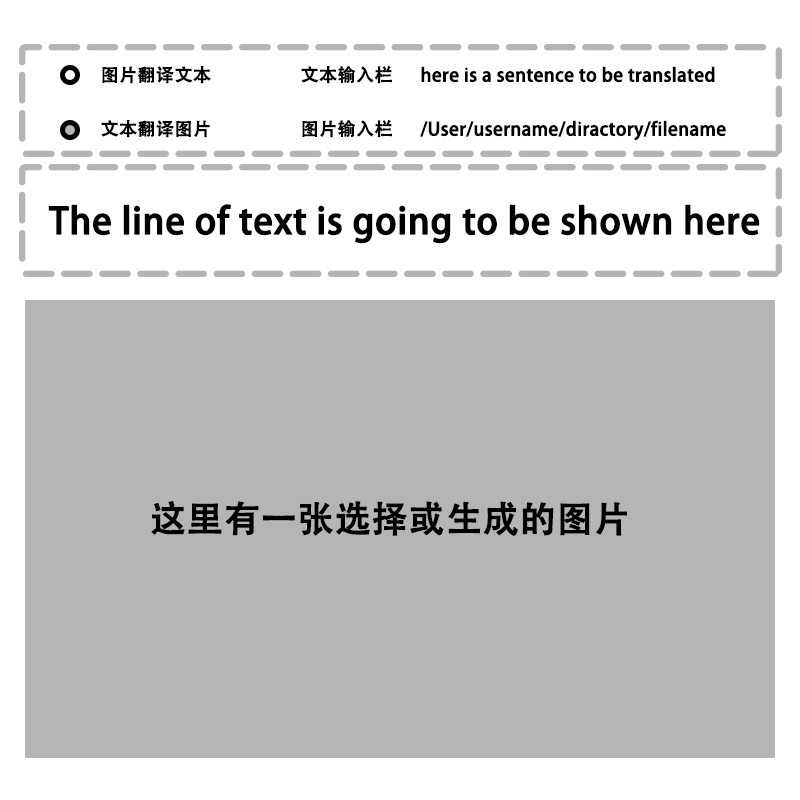
\includegraphics[width=0.8\textwidth]{figures/界面原型图.png}
    \caption{软件界面原型图}
    \label{fig:UIproto}
  \end{figure}

  其中,界面上方由一组两个单选选项的选择栏和两个数据输入栏组成。选项栏的作用是选择当前需要实现的功能,由“图片翻译语义”和“文本翻译图片”两个选项组成;数据输入栏分别是一个文本输入栏和一个文件选择栏,分别对应着文本和图片的输入选择。

  其下是一个明显的按钮,突出的设计可以让用户能轻易明白操作方法,也让用户更有仪式感,能感受到这一操作的划时代意义。

  最下方的大区域是输出区域,根据功能的不同可以输出不同的内容。在选择图像翻译语义功能时,会输出一句话,这一行文字和图片将一起显示,方便对比观察;在选择语义生成图像选项时,将输出生成的图片和原语句,也是为了方便用户观察与分享,表意清晰。

\section{软件功能设计}
功能部分分为图片标注功能以及文字生成图像功能,两个功能我使用了两个结构相对复杂的深度学习模型组合构架的算法,将在下面具体介绍。
 
\subsection{图片标注方法}
\subsubsection{算法整体模型}
在这一模型中,要使用LSTM模型进行训练,训练出的模型放在主函数的调用函数中,实现图片翻译为自然语言的功能。

这一模型主要流程由四步组成。

\begin{enumerate}[fullwidth,itemindent=2em,label=\arabic*.]
    \item 在模型中输入图片,作为输入信息;
    \item 由卷积神经网络提取图片信息,形成图片特征信息(即后文编码步骤);
    \item 由注意力机制(attention)对所提取的图片特征信息进行处理,加强或抑制部分区域,作为后续输入LSTM的输入信息——在不同时刻,注意力信号会受到上一次LSTM的输出信息的影响,即注意力信号作为LSTM神经元细胞的状态,受到输出词语的影响而改变(这也是后文的解码部分);
    \item LSTM最终输出文本,形成最后的结果。
\end{enumerate}

\subsubsection{编码部分}
第一步,要对训练集中的标注编码,形成特征向量。词典中已经预先确定了$K$个词语,对于每一行标注$y_i$,可以将其通过词典序号,将句子映射成输入向量,每一个元素的位置意义是序号,即图片相关的类别,数字则是关联度。编码之后生成向量$\textbf{y}_i$,一起构成输入矩阵。
$$y = {\textbf{y}_1, \textbf{y}_2, ..., \textbf{y}_C}, \textbf{y}_i\in \mathbb{R}^K$$

第二步,对图片编码。使用一个卷积神经网络(Convolutional Neural Network, CNN)对图片的特征进行提取,从而形成图片编码。编码好的图片,后续会作为注释向量$\textbf{a}$使用。
$$a = \{\textbf{a}_1, \textbf{a}_2, ... , \textbf{a}_L\}, \textbf{a}_i \in \mathcal{R}^D$$

\subsubsection{解码部分}
解码部分实用的技术是LSTM,即长短期记忆模型。解码后生成的是标注文本,在预测最后一个词的时候,需要背景向量、前一时刻的隐藏层向量、前一时刻的词。

背景向量$\hat{z}_t$由注意力机制函数和图片注释向量计算得出,并且与时序$t$有关,随时序推进而变化。相当于是有选择地传输图片注释向量中的信息,是图片信息的动态表达。

确定一个注意力机制函数$\phi$来计算$t$时刻的背景向量$\hat{z}_t$。对于输入的图片注释信息,为了推测这一位置是否是正确的注意力集中点,在式\eqref{eq:归一a}中定义一个可以归一化的参数$\alpha_{t,i}$来表示在$t$时刻,位置$i$是正确关注点的置信度。
这个置信度由,计算背景向量
\begin{equation}
    e_{t,i}=f_{att}(\textbf{a}_i,\textbf{h}_t)
\end{equation}
\begin{equation}
    \label{eq:归一a}
    \alpha_{t,i}=\frac{\exp e_{t,i}}{\sum_{k=1}^{L}\exp e_{t,k}}
\end{equation}

计算出权重之后,即可使用注意力机制函数计算出背景向量$\hat{z}_t$:
\begin{equation}
    \hat{z}_t=\phi(\textbf{a}_i,\alpha_i)
\end{equation}

这里的函数$\phi$是利用了软注意力机制\upcite{bahdanau2014neural},这一机制
\subsubsection{代码实现模块}


\subsection{自然语言生成图片方法}
这一模型主要是用通过场景生成图像的GAN模型来训练,得到的模型放在主函数的调用函数中,实现自然语言生成图片的功能。


\subsubsection{代码实现模块}

\begin{algorithm}[H]
    \setstretch{1.5} % 代码间行距设定
    \SetAlgoLined
    \KwResult{Write here the result }
     initialization\;
     \While{While condition}{
      instructions\;
      \eIf{condition}{
       instructions1\;
       }{
       instructions3\;
      }
     }
    \caption{How to write algorithms}
  \end{algorithm}
\section{本章小结}
本章具体地介绍了这一设计中所包含的设计细节及其理论依据,并确定了软件构架的结构,为完成代码构建和实验设计打下了基础。

本章中,确定了以python语言的tkinter库来写界面,保证界面简单简介易懂;用CNN和LSTM技术,基于注意力的方法,通过编码-解码的流程来完成图片标注功能;用基于位置场景的方法,由GNN和两个判别器构成的GAN模型来分步生成图片,最后生成合成图片的方法来实现由文本生成图片的功能。

在下一章里,我会继续记述实验的过程及其表现。
%{\songti \bfseries 宋体加粗} {\textbf{English}}

%{\songti \itshape 宋体斜体} {\textit{English}}

%%%{\songti \bfseries \itshape 宋体粗斜体} {\textbf{\textit{English}}}

%\section{编译}
%本模板必须使用XeLaTeX + BibTeX编译,否则会直接报错。 本模板支持多个平台,结合sublime/vscode/overleaf都可以使用。